\onehalfspacing

%%CAPITOLO 2: =======================================

\chapter{Word cloud statiche}

Questo capitolo consiste in una breve introduzione al concetto di word cloud.

Nella sezione \ref{wc_stat:def} verranno introdotte alcune definizioni e si parler� brevemente di qualche applicazione, mentre nella sezione \ref{wc_stat:arte} si far� il punto sullo stato dell'arte riguardo le word cloud semantiche.

\section{Definizioni e applicazioni}\label{wc_stat:def}
\subsection{Cos'� una word cloud?}
Il recente sviluppo di Internet, con l'avvento del Web 2.0, assieme al grande progresso tecnologico dei calcolatori, ha comportato un'ingente produzione di dati sul web e sulle piattaforme web-based, per cui il problema di estrarre, gestire e visualizzare efficacemente tale informazione � diventata, negli ultimi anni, un'area di ricerca piuttosto importante nella visualizzazione dell'informazione. 

In generale, una \textbf{word cloud} � una rappresentazione visuale di documenti testuali, che utilizza diversi colori, font e dimensioni per raffigurare le parole pi� rilevanti, dette \textbf{keywords}, di un generico documento. Esse sono utilizzate, quindi, per esaminare un testo, in modo da facilitarne la comprensione, o per confrontare pi� testi. Ad esempio, nelle elezioni presidenziali del 2008 e del 2012 (fig. \ref{fig:obama_romney}), i media americani hanno confrontato le word cloud generate dai dibattiti dei candidati alla presidenza americana, mettendo in risalto le differenze tra i discorsi dei candidati; anche in Italia, in occasione del discorso di insediamento alla Camera da parte del presidente Mattarella, alcune testate giornalistiche hanno fatto uso delle word cloud per visualizzare sinteticamente il contenuto del suo discorso (fig. \ref{fig:mattarella}). 
\begin{figure}
\centering
\subfigure[Word cloud generata dal discorso di Obama.]
{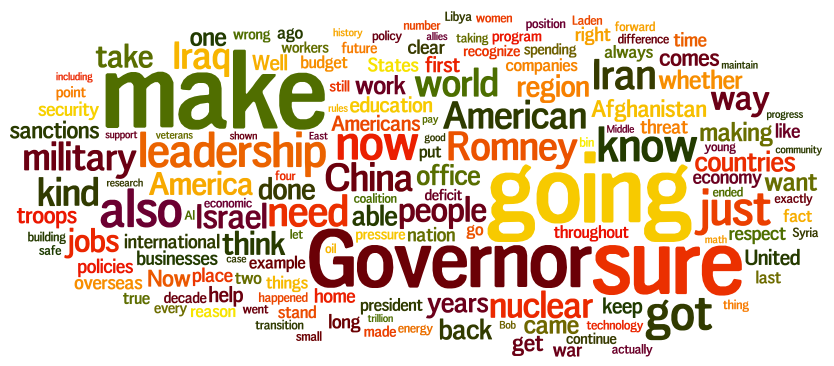
\includegraphics[scale=0.5]{img/wc_statiche/obama_wc.png}}
\hspace{3mm}
\subfigure[Word cloud generata dal discorso di Romney.]
{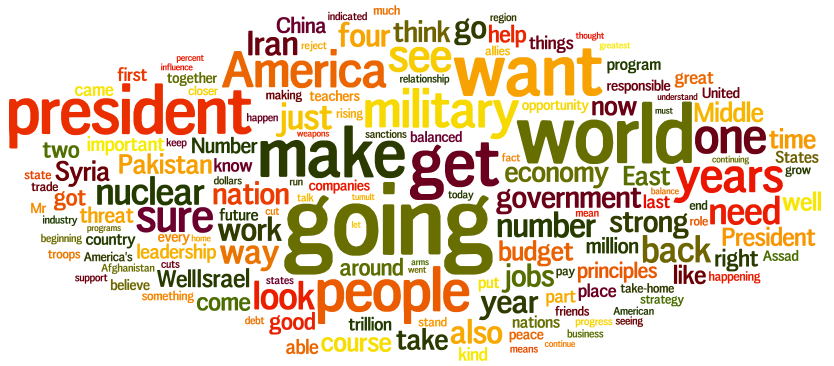
\includegraphics[scale=0.5]{img/wc_statiche/romney_wc.png}}
\caption[Due word cloud relative ai dibattiti tra i candidati alla presidenza statunitense.]{Due wordcloud relative ai dibattiti tra i candidati alla presidenza statunitense.}
\label{fig:obama_romney}
\end{figure}
\begin{figure}
\centering
{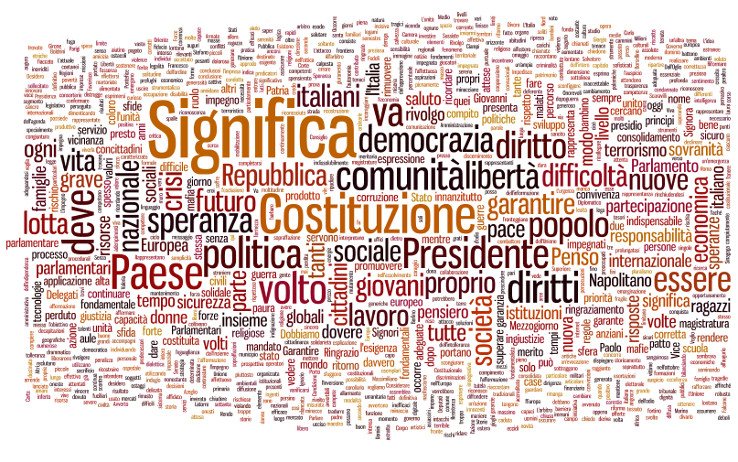
\includegraphics[scale=0.55]{img/wc_statiche/mattarella_wc.png}}
\caption[Word cloud del presidente Mattarella.]{Word cloud del presidente Mattarella.}
\label{fig:mattarella}
\end{figure}

In riferimento al web, si parla invece di \textbf{tag cloud}, con evidente richiamo ai tag. Un tag � un metadato, rappresentato da una parola chiave e riferito ad una specifica risorsa web. Il tag consente la catalogazione dei dati in internet, facilitando la ricerca di una risorsa in base alla sua descrizione. Il loro utilizzo si � diffuso grazie al sito di \textit{photo sharing} Flickr\cite{flickr}, in cui i tag classificano in diverse categorie le foto che vengono condivise dagli utenti.

La word cloud, dunque, costituisce un potente mezzo che consente agli utenti di avere un'intuizione sul contenuto di un documento. Negli anni, sono state sviluppate varie applicazioni che generano word cloud, ognuna con pregi e difetti. Le word cloud tradizionali, cio� le prime ad essere realizzate, dispongono le parole in maniera randomica o in ordine alfabetico. Tuttavia, esse non sono utili, ad esempio, per comparare pi� testi. In tal caso, infatti, gli utenti dovrebbero analizzare manualmente le due visualizzazioni per notare eventuali differenze, e ci� va ad annullare i benefici che ne derivano dall'utilizzo delle word cloud. 

Recentemente, la maggior parte dei tool che genera word cloud si � posta come obiettivo quello di raggruppare semanticamente le parole estratte, utilizzando tecniche di elaborazione del linguaggio naturale per correlare parole simili tra loro. La possibilit� di disegnare, vicine nella word cloud, parole correlate semanticamente, pu� aggiungere informazione utile all'utente, come notato da Deutsch et al. in \cite{Deutsch}. Il raggruppamento semantico delle parole, infatti, aiuta l'utente a comprendere pi� efficientemente il contenuto della word cloud: invece che analizzare le parole singolarmente, l'utente pu� semplicemente dare un rapido sguardo ai gruppi di parole.

Le word cloud hanno diverse caratteristiche: ci� che viene notato immediatamente dall'utente � la dimensione delle parole. Infatti, le parole di una word cloud sono tipicamente pesate in base all'importanza che esse ricoprono nel testo: pi� le parole hanno un font grande, pi� sono rilevanti. In questo modo, le word cloud permettono di evidenziare ci� che � importante in un testo. Ci sono anche altri parametri da tenere in considerazione. In \cite{halvey}, Halvey e Keane hanno valutato l'effetto di alcuni fattori: la posizione delle parole, la loro disposizione secondo l'ordine alfabetico e, come detto, la dimensione del font, si sono rivelati parametri importanti. Inoltre, hanno notato che gli utenti, piuttosto che leggere tutte le parole, danno uno sguardo generale alla word cloud. In un altro lavoro, Lohmann et al.\cite{Lohmann} hanno scoperto che parole posizionate vicino al centro catturano di pi� l'attenzione rispetto a parole vicine ai bordi, cos� come parole posizionate in alto a sinistra vengono percepite prima delle altre da parte degli utenti. 

Ad ogni modo, le word cloud non devono mirare troppo ai soli parametri estetici, cio� non devono avere troppi colori, parole con diverse orientazioni ecc... Dovendo fornire all'utente informazione in breve tempo ed in maniera intuitiva, devono essere pi� semplici e chiare possibile.

\subsection{Applicazioni}
I contesti applicativi delle word cloud sono molteplici. Esempi di applicazioni, come detto, riguardano l'analisi e la comparazione di testi scritti, ma anche:
\begin{itemize}
\item analisi statistiche relative ad un sito web: parole chiave utilizzate nei motori di ricerca che hanno condotto al sito web, statistiche relative ai visitatori (ad esempio, il paese di provenienza o le sezioni pi� cliccate); 
\item analisi dei \textit{trending topic}, tramite \textit{hashtag}, dei vari social network (Twitter, Facebook, ecc...); 
\item la visualizzazione dei risultati di un motore di ricerca;
\item utilizzo didattico come strumento di apprendimento per gli studenti; 
\item ecc..
\end{itemize}
Le word cloud, quindi, costituiscono strumenti utili per fornire all'utente un'informazione sommaria su dei dati. Poi sta all'utente analizzarne il contenuto e ricavarne pi� informazione possibile.
\section{Stato dell'arte}\label{wc_stat:arte}
Esistono diversi strumenti per la creazione di word cloud. Un tool web-based molto popolare, Wordle\cite{Viegas:2009}, grazie alle qualit� grafiche e alle sue funzionalit�, ha permesso la diffusione delle word cloud come potente strumento per riassumere e analizzare un testo. Con Wordle, ad esempio, � possibile impostare alcuni parametri in modo da personalizzare la word cloud finale, come il numero delle parole, il colore, gli angoli di disegno ecc.. Tuttavia, Wordle non riesce a catturare le relazioni semantiche tra le parole, propriet� che pu� rivelarsi cruciale nell'analisi e nella comprensione di un testo. 
Per ovviare a ci�, � stato proposto un ulteriore strumento, basato su Wordle, chiamato ManiWordle\cite{kohk}, il quale offre un buon livello di interazione con l'utente, permettendo a quest'ultimo di manipolare il disegno finale e di modificare le parole visualizzate in termini di posizione, colore e orientamento, risultando quindi pi� flessibile di Wordle. Un altro sistema, SparkClouds\cite{lee}, tramite l'uso delle \textit{sparklines}, mette in risalto i cambiamenti tra pi� word cloud. Collins et al.\cite{collins}, hanno presentato Parallel Tag Clouds, uno strumento in grado di visualizzare le differenze tra i testi scritti di un ricco dataset. FacetAtlas\cite{facetatlas}, invece, � un'applicazione che, tramite grafici e mappe di densit�, visualizza le relazioni che intercorrono tra i documenti di una vasta collezione di testi.
Tree Cloud\cite{gambette}, � un tool in cui le parole vengono disposte secondo un albero, in modo tale da preservare la loro vicinanza semantica. In \cite{cui}, Cui et al., tramite misure di similarit�, mirano a collocare, vicine nel disegno, parole correlate semanticamente, utilizzando poi un metodo force directed per compattare la word cloud. Wu et al.\cite{seam}, utilizzano una tecnica ispirata al \textit{seam carving}, algoritmo di ridimensionamento dell'immagine in base ai contenuti, per ottenere una word cloud semantica e compatta. Questo lavoro di tesi, invece, prende spunto dal recente lavoro svolto da Kobourov et al.\cite{kobourov}, in cui vengono implementati due nuovi algoritmi di visualizzazione, da confrontare con altri algoritmi esistenti, per analizzare la qualit� delle word cloud in base a diverse metriche, ovviamente partendo dalla base comune costituita dalla coerenza semantica nella disposizione delle parole. 